
\documentclass{beamer}
\mode<presentation>
{
  \usetheme{default}      % or try Darmstadt, Madrid, Warsaw, ...
  \usecolortheme{default} % or try albatross, beaver, crane, ...
  \usefonttheme{default}  % or try serif, structurebold, ...
  \setbeamertemplate{navigation symbols}{}
  \setbeamertemplate{caption}[numbered]
}
\usepackage[spanish]{babel}
\usepackage[utf8x]{inputenc}

\title[Clase 2]{Procesamiento de bases de datos con STATA}
\subtitle{Clase 2}
\author{Claudia Vazquez}
\date[]{\texttt{clauvazqu@gmail.com}\\Centro REDES}
\pgfdeclareimage[height=0.5cm]{university-logo}{logo-redes}
\logo{\pgfuseimage{university-logo}}

\begin{document}

\begin{frame}
  \titlepage
\end{frame}

\begin{frame}{Contenido}
  \tableofcontents
 \end{frame}

\section{Sinxtaxis}

\begin{frame}[allowframebreaks]{Sintaxis básica de los comandos}
Los comandos son un lenguaje de comunicación con STATA, por lo que \underline{deben respetar una sintaxis}. La sintaxis general es:\\
\medskip
{\footnotesize [by \textit{varlist}:] \texttt{command} [\textit{varlist}] [=\textit{exp}] [if \textit{exp}] [in \textit{range}] [\textit{weight}] [, \textit{options}]}\\
\medskip
donde:
\begin{itemize}
\item 
\begin{itemize}
\item \textit{varlist}: lista de variables.
\item \textit{exp}: expresión algebraica.
\item \textit{range}: rango de observaciones. 
\item \textit{options}: lista de opciones. 
\item \textit{weight}: expresión para ponderar que veremos más adelante.
\end{itemize}
\item Los corchetes distinguen entre elementos opcionales y obligatorios: lo que esté entre corchetes es opcional.
\item El \texttt{help} de cada comando explicita cuál es su sintaxis específica (elementos opcionales y obligatorios) y qué opciones admite (se especifican después de una coma). 
\item Para verlo simplemente tipeamos \texttt{help} más el nombre del comando y se abrirá una nueva ventana.
\item Si un elemento no está en la sintaxis de un comando particular, implica que el comando no lo admite.
\item A continuación veremos ejemplos para ilustrar cada una de las partes de la sintaxis. Tener siempre presente la estructura general:
\end{itemize}
{\footnotesize [by \textit{varlist}:] \texttt{comand} [\textit{varlist}] [=\textit{exp}] [if \textit{exp}] [in \textit{range}] [\textit{weight}] [, \textit{options}]}
\end{frame}

\begin{frame}{Ejemplo: comando summarize}{}
{\footnotesize Si tipeamos \texttt{help summarize} en la línea de comandos se abre la ventana:}
\centerline{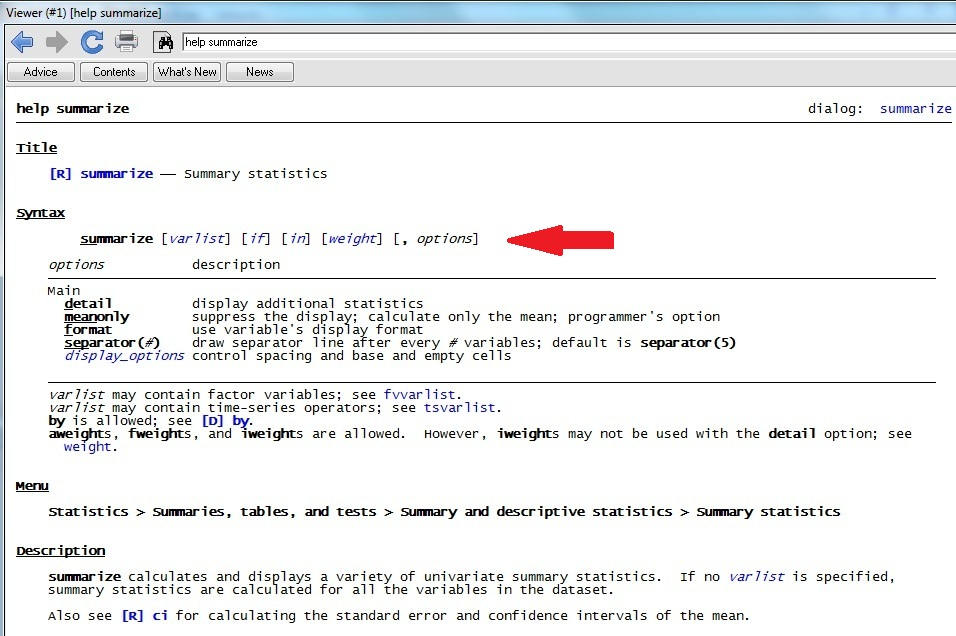
\includegraphics[height=6.8cm]{summ.jpg}}
\end{frame}
\subsection{varlist}
\begin{frame}{Sintaxis}{Ejemplos de usos de [varlist]}
\begin{itemize}
\item Ahí vemos que \textit{varlist} aparece entre corchetes, indicando que es opcional: el comando puede utilizarse con o sin una \textit{varlist}. Es decir:
\begin{itemize}
\item Podemos escribir \texttt{summarize} en la línea de comandos sin especificar una lista de variables y obtendremos una tabla con estadísticas descriptivas para \underline{todas las variables}.  
\item O podemos especificar a qué variable/s queremos que se aplique el comando:
\begin{itemize} 
\item  \texttt{summarize weight} \hspace{0.3 cm} $\rightarrow$  Calcula estadísticas descriptivas para la variable ``weight''.
\item \texttt{summarize mpg rep78 turn} \hspace{0.3 cm} $\rightarrow$  Calcula estadísticas descriptivas para las variables ``mpg'', ``rep78'' y ``turn''.
\item  \texttt{summarize p*}  \hspace{0.3 cm} $\rightarrow$ calcula estadísticas descriptivas para todas las variables que comienzan con ``p''. 
\end{itemize}
\end{itemize}
\end{itemize}
\end{frame}

\subsection{if/in}
\begin{frame}[allowframebreaks]{Sintaxis}{Ejemplos de usos de [if exp]}
\begin{itemize}
\item La aplicación de un comando puede restringirse a observaciones que cumplan con determinadas condiciones. 
\item Para especificar un condicional existen: 
\begin{itemize}
\item Operadores de comparación: == (igual), != (distinto), $>$, $<$, $>=$, $<=$ (mayor, menor, mayor o igual, menor o igual)
\item Operadores lógicos: \& (``y''), $|$ (``o''), ! (``no'')
\item El paréntesis determina el orden de aplicación de las sentencias.
\end{itemize}
\item Ejemplos:
\begin{itemize} 
\item \texttt{tabulate rep78 if foreign==0}  \hspace{0.3 cm} $\rightarrow$ produce la tabla de frec. de ``rep78'' para autos nacionales.
\item \texttt{tabulate rep78 if price $>$6165.257 \& foreign==0}  \hspace{0.3 cm} $\rightarrow$ produce la tabla de frec. de ``rep78'' para autos con precio mayor al promedio y nacionales.
\item  \texttt{summarize length if length $<$ 180 $|$ weight $>$ 3400}  \hspace{0.3 cm} $\rightarrow$ estadísticas de la variable ``lenght'' para autos con longitud menor a 180 o peso mayor a 3.400.
\item  \texttt{tabulate foreign if price !=0}  \hspace{0.3 cm} $\rightarrow$ produce tabla de frec. de la variable ``foreign'' para autos con precio distinto de cero.
\end{itemize}
\item Notar el doble signo (``=='') para denotar igualdad en este caso. Un solo signo igual se usa únicamente para asignar un valor a una variable (\texttt{generate} o \texttt{replace}).
\item Los comandos aceptan un único \textit{if}: luego las condiciones se combinan con el ``y'' (\&) y/o con el ``o'' ($|$).
\end{itemize}
\end{frame}


\begin{frame}{Sintaxis} {Ejemplos de usos de [in range]}
\begin{itemize}
\item La aplicación de los comandos puede restringirse también a un rango de observaciones, de acuerdo al orden de la base de datos:
\begin{itemize}
\item  \texttt{summarize price in 1/10}  \hspace{0.3 cm} $\rightarrow$ el comando se aplica a las diez primeras observaciones.
\item  \texttt{summarize price in -10/-1} \hspace{0.3 cm} $\rightarrow$ el comando se aplica a las últimas diez observaciones.
\end{itemize}
\item La aplicación de [in \textit{range}] depende del orden de la base.
\item El comando para ordenar una base de datos es \texttt{sort} (orden ascendente). Luego debe especificarse la/s variable/s por las que se ordenará la base.
\end{itemize}
\end{frame}


\begin{frame}{Sintaxis}{Ejemplos del uso de [=exp]}
\begin{itemize}
\item Con [= exp] se asigna un valor a una variable.
\item El uso más frecuente es con \texttt{generate} y \texttt{replace}.
\item \texttt{generate} permite crear una variable nueva, para la que es necesario indicar el valor que va a tener:
\begin{itemize}
\item \texttt{generate var1=2} \hspace{0.3 cm} $\rightarrow$ Crea una variable llamada ``var1'' que tiene valor 2 en todas las observaciones.
\item \texttt{generate mpg2= mpg\^{}2}  \hspace{0.3 cm} $\rightarrow$ Crea una variable llamada ``mpg2'' que es igual al valor de ``mpg'' al cuadrado.
\item  \texttt{generate miss= .}  \hspace{0.3 cm} $\rightarrow$ Crea una variable llamada ``miss'' con todos los valores faltantes (\textit{missing}).
\end{itemize}
\item El comando \texttt{replace} permite reemplazar valores de una variable ya existente:
\begin{itemize}
\item \texttt{replace mpg2 = 0 if price $==$0}  \hspace{0.3 cm} $\rightarrow$  reemplaza por un 0 a ``mpg2'' en aquellas observaciones que tengan valor de ``price'' igual a 0.
\end{itemize}
\end{itemize}
\end{frame}


\subsection{by varlist}

\begin{frame}{Sintaxis}{Ejemplos de usos de [by varlist:]}
\begin{itemize}
\item El uso del prefijo [by \textit{varlist}:] permite aplicar el comando por grupos, definidos por los valores de la variable indicada a continuación del \textit{by}.
\item Para aplicar el prefijo [by \textit{varlist}:] es requisito que la base esté ordenada por la/s variable/s del \textit{by}. 
\item Con \texttt{by foreign: summarize price} el comando \texttt{summarize} se ejecuta por separado para los distintos valores de ``foreign''.
\end{itemize} 
\centerline{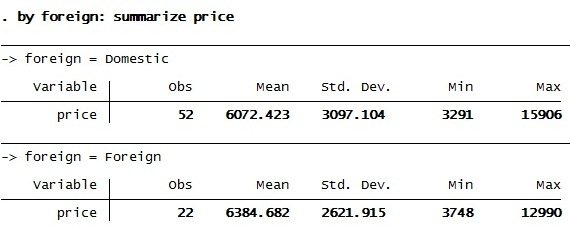
\includegraphics[height=2.5cm]{by.jpg}}
\end{frame}

\begin{frame}{Sintaxis}{Ejemplos de usos de [by varlist:]}
\begin{itemize}
\item En el ejemplo anterior, la base auto.dta ya estaba ordenada por la variable ``foreign'' (esto lo podemos constatar con el comando \texttt{describe}).
\item Si hubiéramos querido aplicar el comando para los distintos valores de otra variable, por ejemplo ``rep78'', hubiéramos obtenido un error:\\\medskip
\centerline{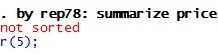
\includegraphics[height=1cm]{byrep.jpg}}
\item Para poder hacerlo, o se ordena primero la base con el comando \texttt{sort rep78} o se utiliza directamente el comando \texttt{bysort rep78: summarize price}.
\end{itemize}
\end{frame}

\begin{frame}{Sintaxis}{Ejemplos de usos de [by varlist:]}
\centerline{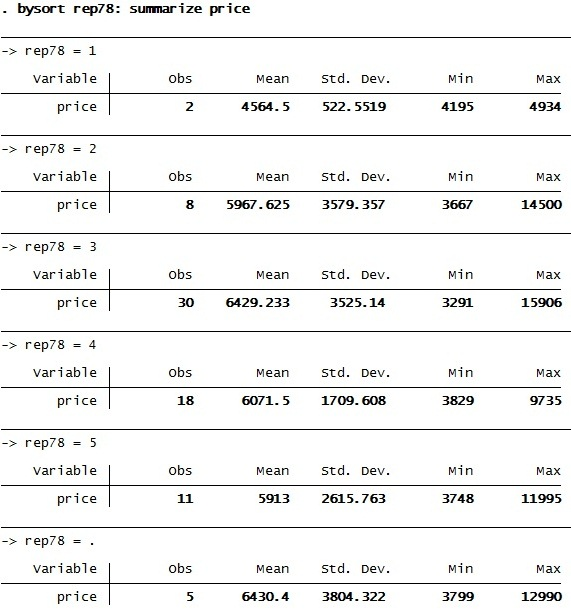
\includegraphics[height=6.5cm]{bysort.jpg}}
\end{frame}


\subsection{options}

\begin{frame}{Sintaxis}{opciones}
\begin{itemize}
\item Los comandos suelen aceptar opciones, que se describen en el \texttt{help} de cada comando:\\
\centerline{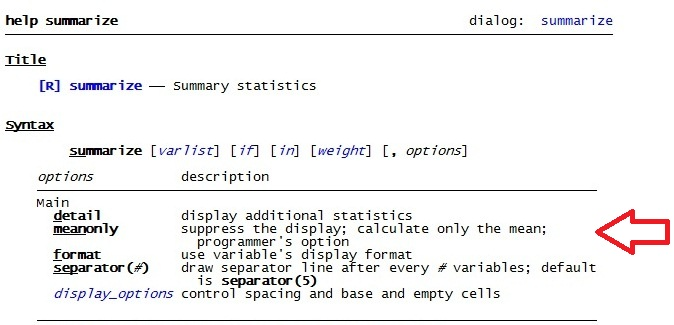
\includegraphics[height=2.2cm]{option.jpg}}
\item El comando \texttt{summarize} acepta las opciones: \texttt{detail, meanonly, format y separator}: 
\begin{itemize}
\item \texttt{summarize price, detail} \hspace{0.3 cm} $\rightarrow$  Presenta estadísticos adicionales.
\item \texttt{summarize price, meanonly} \hspace{0.3 cm} $\rightarrow$  Suprime el display del resultado y no calcula la varianza. 
\end{itemize}
\end{itemize}
\end{frame}

\begin{frame}{Abreviaturas}
\begin{itemize}
\item STATA permite abreviar los nombres de comandos, opciones y variables.
\item En las clases evitamos las abreviaturas para mejorar la compresión, pero son muy prácticas.
\item La regla general es que la abreviatura puede realizarse siempre que no se confunda con otro comando/variable.
\item Cuando un comando puede abreviarse se indica en el syntax del \texttt{help} subrayando de la cantidad mínima de letras que deben escribirse: \texttt{\underline{su}mmarize} indica que puede escribirse \texttt{``su''}.
\item Los comandos ``destructivos'', que implican pérdida de datos (como \texttt{clear}, \texttt{drop}), no pueden abreviarse.
\end{itemize}
\end{frame}

\section{Tipos de datos}

\begin{frame}{Tipos de datos}
\begin{itemize}
\item Los tipos de datos que puede almacenar STATA son tres: 
\begin{itemize}
\item Números
\item Texto (se denominan \textit{string})
\item Fechas
\end{itemize}
\item Para conocer el tipo de datos de las variables en la base puede utilizarse el comando \texttt{describe}.
\end{itemize}
\end{frame}

\subsection{números}

\begin{frame}[allowframebreaks]{Tipos de datos numéricos}
Los tipos de variables numéricas en STATA  son:\\\medskip
\begin{tabular}{c c c c}
\hline
{\footnotesize Storage type}& {\footnotesize Tipo número}&{\footnotesize Límite inferior}& {\footnotesize Límite superior}\\\hline
{\footnotesize byte}& {\footnotesize Enteros} &{\footnotesize $-127$} &{\footnotesize $+100$}\\
{\footnotesize integer} &{\footnotesize Enteros}&{\footnotesize $-32.767$} &{\footnotesize $+32.740$}\\
{\footnotesize long} &{\footnotesize Enteros}&{\footnotesize $-2.147.483.647$} &{\footnotesize $+2.147.483.620$}\\
{\footnotesize float} &{\footnotesize Con decimales}&{\footnotesize $-1.70 x 10^{38}$}&{\footnotesize $+1.70 x 10^{36}$}\\
{\footnotesize double}& {\footnotesize Con decimales}&{\footnotesize $-8.99 x 10^{307}$}&{\footnotesize $+8.99 x 10^{308}$}\\\hline
\end{tabular}
\begin{itemize}
\item Por defecto, cuando se genera una variable numérica STATA le asigna el tipo \textit{float} (puede implicar un desperdicio de memoria). 
\item Para crear la variable ``var1'' especificando el tipo (por ej. byte) se utiliza: \texttt{generate byte var1=0}.
\item Si luego se ingresan datos que no se corresponden con ese tipo, STATA lo cambia automáticamente:\\
\centerline{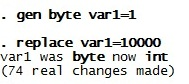
\includegraphics[height=1.2cm]{byte.jpg}}
\item Cuando una variable numérica tiene valor \textit{missing} se muestra con un punto (.)
\item STATA considera al missing como el valor numérico más alto: si escribimos \texttt{browse if rep78>=4} nos va a mostrar las observaciones que tengan ``rep78'' igual a 4, a 5 o missing.
\item Las operaciones algebraicas que involucran a algún missing tienen missing como resultado (missing no es cero!).
\end{itemize}
\end{frame}

\subsection{texto}

\begin{frame}{Tipos de datos \textit{string}}
\begin{itemize}
\item Un \textit{string} es una secuencia de caracteres entre comillas dobles (`` ''). Las comillas no se consideran parte del  \textit{string} sino que lo delimitan.
\item Los espacios y mayúsculas importan: ``hola'' es diferente a `` hola'', a ``hola '' y a ``Hola''.
\item En las variables \textit{string} el missing es ``'', no un punto.
%\item Se pueden almacenar \textit{string} de hasta un máximo de 244 caracteres (STATA 11).  
\item Las variables \textit{string} pueden contener:
\begin{itemize}
\item Datos \underline{identificatorios}, tales como nombres de pacientes, ciudades, marcas, etc., que no se utilizan \textit{directamente} en análisis estadísticos.
\item Datos de \underline{categorías}, como sexo, que puede estar codificado como ``masculino''/``femenino''. En este caso, puede ser conveniente asignar un código y almacenar la variable como numérica. 
\end{itemize}
\end{itemize}
\end{frame}

\begin{frame}{Tipos de datos \textit{string}}{comando \texttt{encode}}
\begin{itemize}
\item El comando \texttt{encode} crea una nueva variable numérica en base a una \textit{string} y le asigna una etiqueta a cada valor de acuerdo a la palabra almacenada en el \textit{string}.
\item Por ejemplo, si tenemos una variable llamada ``sexo'' que toma valores ``fem'' y ``masc'' escribiendo \texttt{encode sexo, gen(sex)} creamos una nueva variable (``sex'') que toma los valores 1 y 2.
\item Cada uno de esos valores tendrá asociada la etiqueta que corresponda (``fem'' o ``masc'').
\item Si una variable almacenada como \textit{string} contiene en realidad números se puede convertir a numérica con el comando \texttt{destring} (no usar \texttt{encode} en este caso).
\end{itemize}
\end{frame}


\subsection{fechas}

\begin{frame}{Tipos de datos fechas}
\begin{itemize}
\item STATA representa las fechas con un número entero que indica la cantidad de unidades de tiempo (días, semanas, meses, etc.) que transcurrieron desde un momento de referencia, fijado en el 1ro de enero de 1960.
\item Por ejemplo, si la unidad de tiempo fueran días (formato \%td) o meses (formato \%tm), la interpretación de los valores numéricos sería la siguiente:
\end{itemize}
{\footnotesize
\begin{center}
\begin{tabular}{p{1.7cm} p{1.7cm} p{1.5cm} } 
\hline
 & \multicolumn{2}{ c }{Interpretación}\\
Valor & \multicolumn{2}{ c }{Unidad de tiempo}\\
 numérico& días & meses\\\hline
0& 01jan1960&1960m1\\
1& 02jan1960&1960m2\\
-3& 30dec1959&1959m10\\
4.569 & 05jul1972&2340m10\\
-4.569&29jun1947&1579m4 \\
\hline
\end{tabular}
\end{center}}
\end{frame}


\begin{frame}[allowframebreaks]{Tipos de datos fechas}
\begin{itemize}
\item Existen funciones para transformar variables \textit{string} que contienen fechas a valores numéricos que STATA puede interpretar como fechas y realizar operaciones.
\item Supongamos que cargamos una base de datos que contiene la variable ``fecha'' con los siguientes valores:\\\medskip
\centerline{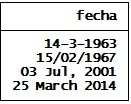
\includegraphics[height=2cm]{fecha.jpg}}
\item Esa variable es un \textit{string}: contiene caracteres no numéricos como ``-'' ``/'', ``,'', ``Jul'' y ``March''. 
\item Ahora creamos una variable numérica (``fecha1'') que STATA pueda interpretar como fecha. 
\item Como la variable original representa un día utilizamos la función \texttt{date()}. Además, le indicamos que el orden en que vienen los datos es: día, mes y año (con ``DMY'', que se denomina \textit{mask}):\\
\texttt{generate fecha1=date(fecha, ``DMY'')}
\item El resultado es una variable que contiene la cantidad de días transcurridos desde el 01/01/1960.\\\medskip
\centerline{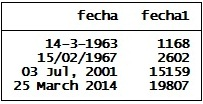
\includegraphics[height=2cm]{fecha1.jpg}}
\item Como vemos, la función \texttt{date()} puede interpretar distintas formas de fecha dentro de un \textit{string}: algunos campos tenían guiones, otros barras, etc.
\item Existen distintas funciones, dependiendo de cómo estén expresadas las fechas (ver \texttt{help date}).
\item Si el dato original hubiera sido del tipo ``21aug2005 15:21:22'', hubiéramos usado la función \texttt{clock()} con el \textit{mask} ``DMYhms'' (para indicar que el orden de los elementos es: día, mes, año, hora, minutos, segundos):\\
\texttt{generate fecha1=clock(fecha, ``DMYhms'')}
\item La ventaja de tener fechas con el tipo de variable correcto es que podemos realizar distintas operaciones. 
\item Por ejemplo, supongamos que recibimos una base de datos de un hospital con la siguiente información para cada paciente:\\\medskip
{\footnotesize
\begin{center}
\begin{tabular}{p{2cm} p{2cm}}
\hline
ingreso&egreso\\\hline
21 May 2012& 30 May 2012\\
21 May 2012& 25 May 2012\\
23 May 2012& 02 Jun 2012\\
24 May 2012& 10 Jun 2012\\
...&...\\
\hline
\end{tabular}
\end{center}}
\item Queremos crear una variable con la cantidad de días que permaneció internado cada paciente.
\item No podemos restar la columna ``egreso'' con ``ingreso'' porque se trata de dos \textit{string}. Lo que hacemos es convertir cada columna en una fecha, y después crear otra variable con la diferencia: \\
\texttt{generate f\_ingreso=date(ingreso, ``DMY'')}\\
\texttt{generate f\_egreso=date(egreso, ``DMY'')}\\
\texttt{gen cant\_dias=f\_egreso - f\_ingreso}
\item El resultado es el siguiente: \\\medskip
\centerline{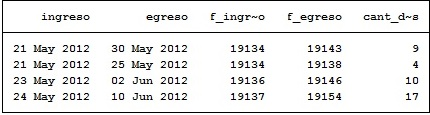
\includegraphics[height=2cm]{dias.jpg}}
\item Existen otras funciones específicas para las fechas. Por ejemplo, a partir de la variable ``f\_egreso'' podemos crear una variable nueva (``mes\_egreso'') que contenga el mes (1-12) en el que el paciente fue dado de alta:\\\smallskip
\texttt{generate mes\_egreso=month(f\_egreso)}
\item El resultado sería:\\\medskip
\centerline{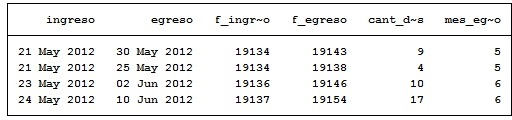
\includegraphics[height=2cm]{mes.jpg}}
\item Por último, supongamos que recibimos una base con una variable fecha expresada de la siguiente manera:\\
\centerline{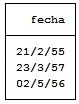
\includegraphics[height=1.6cm]{fecha_a.jpg}}
\item Si intentamos crear la variable numérica con el comando que vimos recién el resultado es missing para todos los valores:\\
\texttt{generate fecha1=date(fecha, "DMY")}
\centerline{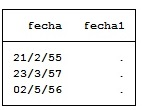
\includegraphics[height=1.6cm]{fecha_a1.jpg}}
\item Esto es porque STATA no puede interpretar si se trata del año 1955 o 2055, etc.
\item La solución consiste en indicar la centuria por defecto: \texttt{generate fecha2=date(fecha, "DM19Y")}\\\medskip
\centerline{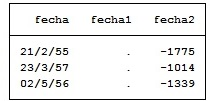
\includegraphics[height=1.6cm]{fecha_a2.jpg}}
\end{itemize}
\end{frame}

\section{Formatos}

\begin{frame}[allowframebreaks]{Formatos}
\begin{itemize}
\item Los formatos permiten determinar cómo se \underline{muestran} las variables numéricas, string y fechas.
\item Con el comando \texttt{describe} vemos el formato que tiene una variable (columna ``display format'') y para cambiarlo usamos \texttt{format}.
\item Los formatos con los que se muestran las variables no modifican la forma en la que están almacenadas.
\item Formatos numéricos:
\begin{itemize}
\item Todos los formatos comienzan con el signo ``\%'' seguido de ``$n_{1}.n_{2}$'' y un caracter que puede ser ``e'', ``f'' o ``g'' (ejemplo: ``\%9.0f''). 
\item $n_{1}$ es el ancho máximo del resultado (cant. de caracteres que se muestran) y $n_{2}$ es la cantidad de decimales.
\item Respecto del las letras, los formatos son ``g'' (formato general), ``f'' (fijo) y ``e'' (notación científica). 
\item En el formato general, STATA decide cuántos decimales va a usar en base al número que se trate. En el fijo, la cantidad de decimales que le asignamos es la que se muestra siempre. 
\item Por ejemplo, en la tabla a continuación se muestra que si $n_{2}$ es igual a 2, el número 1000 se muestra como ``1000.00'' en el formato fijo. Con el formato general omitirían los decimales para ese número (redondo).
\item También vamos que con el formato general la raíz de 2 se muestra con 6 decimales, que sumados al punto y a la parte entera (1) ocupan una longitud de 8 caracteres (el formato se ``reserva'' un espacio más para un posible signo negativo).
\item El número 100,000,000 se lleva a notación científica porque supera el ``ancho'' del formato. Para que se muestre sin esa notación deberíamos aumentar $n_{1}$\\\smallskip
\end{itemize}
\centerline{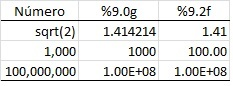
\includegraphics[height=1.6cm]{format.jpg}}
\item  Formatos de fechas
\begin{itemize}
\item Los formatos de fechas comienzan con \%t seguido de un caracter que indica la unidad de tiempo: ``c'' (segundos), ``d'' (días), ``w'' (semanas), ``m'' (meses), ``q'' (trimestres) o ``h'' (semestres).
\item Si a las variables que creamos a partir de las fechas de ingreso y egreso de pacientes les cambiamos el formato con \texttt{format  f\_ingreso f\_egreso \%td} en lugar de los números vemos:\\\medskip
\centerline{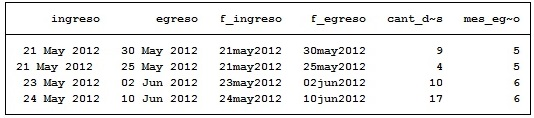
\includegraphics[height=2.2cm]{format2.jpg}}
\end{itemize}
\item Formatos string
\begin{itemize}
\item Los formatos de las variables string tienen la forma \%$n_{1}$s, donde $n_{1}$ es la longitud con la que se muestra el string.
\end{itemize}
\end{itemize}
\end{frame}

\section{Importación de bases de datos}

\begin{frame}[allowframebreaks]{Importación de datos}
\begin{itemize}
\item Cuando tenemos una base en formato .dta la cargamos en STATA con el comando \texttt{use \textit{filename}}.
\item Las bases de datos que no están en formato .dta (formato propio de  STATA) suelen estar en alguno de los siguientes formatos:
\begin{itemize}
\item archivo binario propietario (ej. planillas de cálculo de Excel)
\item base de datos (dBase)
\item programa estadístico (SPSS, SAS)
\item texto plano:
\begin{itemize}
\item fijo 
\item delimitado (por comas, tabulaciones, otros)
\end{itemize}
\end{itemize}
\item En STATA 12 se pueden importar directamente archivos propietarios como hojas de cálculo de Excel con el comando \texttt{import excel} (o desde el menú \textbf{File $>$ Import $>$ Excel spreadsheet}).
\item En STATA 11 y anteriores no pueden abrirse directamente ese tipo de archivos. La alternativa es: 
\begin{enumerate}
\item Abril el archivo en Excel. 
\item Guardar el archivo como texto delimitado por tabulaciones (.txt) o comas (.cvs). Atención a las advertencias respecto a las planillas con múltilpes hojas, dado que solo la hoja activa se almacenará. 
\item Importar desde STATA usando el comando \texttt{insheet}.
\end{enumerate}
\item Otra alternativa es copiar y pegar los datos en el Editor de STATA (que se abre con el comando \texttt{edit}).
\item Si el archivo de texto es de formato fijo o delimitado por espacios, hay que usar el comando \texttt{infile}.
\item También existe un software específico llamado Stat/transfer que convierte las bases de datos de .dta a varios otros formatos y viceversa (no resulta imprescindible tenerlo ya que no hace nada que no pueda hacerse directo desde STATA pero a veces es útil).
\end{itemize}
\end{frame}

\begin{frame}{Problema de la notación decimal}
\begin{itemize}
\item STATA trabaja con notación decimal americana (punto separador decimal) sin importar la configuración regional del sistema operativo.
\item Interpretará como \textit{string} los números separados con comas.
\item Para solucionar esto podemos utilizar la opción \texttt{dpcomma} del comando \texttt{destring}. Suponiendo que en ``var1'' tenemos números con comas almacenadas como texto:\\
\texttt{destring var1, dpcomma replace}\\
\item De esta forma convertimos a ``var1'' en numérica, ignorando la coma decimal.
\end{itemize}
\end{frame}

\begin{frame}{Ejemplo uso \texttt{insheet}}
\begin{itemize}
\item En la plataforma tienen una base de datos con la población, superficie y tasa de analfabetismo de las provincias argentinas (año 2001). 
\item El archivo se llama base\_provincias.xls y está en formato excel. Lo abrimos y guardamos como texto (delimitado por tabulaciones). Supongamos que lo guardamos en la carpeta C: \textbackslash Users \textbackslash Claudia \textbackslash Documents \textbackslash curso redes.
\item Para cargar esta base, desde STATA escribimos:\\
{\footnotesize \texttt{insheet using ``C:\textbackslash Users\textbackslash Claudia\textbackslash Documents\textbackslash curso redes\textbackslash base\_provincias.txt'', tab names}}
\item Con la opción \texttt{tab} indican que el texto está delimitado por tabulaciones. Con la opción \texttt{names}, que el nombre de la variable está en la primera fila.
\end{itemize}
\end{frame}

\end{document}

\begin{frame}{Directorios}
\begin{itemize}
\item Es importante saber en qué directorio estamos, para abrir y guardar archivos sin especificar un \textit{path}:
\begin{itemize}
\item \textbf{save} base.dta  \hspace{0.3 cm} $\rightarrow$ Guarda la base en la carpeta en la que estamos
\item \textbf{save} ``c:\textbackslash clase1\textbackslash base.dta''  \hspace{0.3 cm} $\rightarrow$ Guarda la base en la carpeta c:\textbackslash clase1 
\end{itemize}
\item Para saber en qué carpeta estamos usamos \textbf{pwd}
\item Para cambiar la capeta de trabajo usamos \textbf{cd}:
\begin{itemize}
\item \textbf{cd} ``c:\textbackslash clase1''  \hspace{0.3 cm} $\rightarrow$ Nos posiciona en la carpeta c:\textbackslash clase1 
\end{itemize} 
\item Podemos crear una carpeta de trabajo desde Windows o directamente desde STATA, con \textbf{mkdir}
\item Cuando el nombre de directorios contengan espacios es obligario el uso de dobles comillas. Lo mismo sucede con los nombres de archivos
\end{itemize}
\end{frame}

\section{Comandos básicos}

\subsection{Reportes}

\end{frame}


\subsection{Manipulación de datos}

\begin{frame}{Keep y drop}
\begin{itemize}
\item \textbf{drop} elimina variables u observaciones de los datos en memoria
\item \textbf{keep} hace lo mismo que  \textbf{drop} excepto que hay que especificar las variables u observaciones que queremos conservar, en lugar de las que queremos eliminar
\item \textbf{dropmiss} elimina aquellas variables de la lista de variables para las cuales todas las observaciones tienen valores \textit{missing}
\item Estos comandos no son \underline{reversibles}
\end{itemize}
\end{frame}

\begin{frame}{egen}
\begin{itemize}
\item \textbf{egen} es una extensión del comando \textbf{generate} que incluye muchas funciones creadas por usuarios. Entre otras:
\begin{itemize}
\item \underline{Estadísticas resumen}: count(), max(), mean(), median(), mode(), sd(), total()
\item \underline{Patrones}: fill(), seq()
\item \underline{Funciones a nivel fila}: rowtotal(), rowmean(), rowmiss(), rowmin()
\item \underline{Variables string}: concat(), ends()
\item \underline{Variables categóricas}: anyvalue(), anymatch(), anycount(), group()
\end{itemize}
\item Es muy recomendable leer el \textit{help} del comando \textbf{egen} para conocer todas las funciones
\end{itemize}

\end{frame}


\begin{frame}{Unión de bases de datos}
\begin{itemize}
\item STATA permite unir bases de datos de dos maneras:
\begin{itemize}
\item Con el comando \textbf{merge} se agregan nuevas \textit{variables} a una base existente
\item Con el comando \textbf{append} se agregan nuevas \textit{observaciones} a una base existente
\end{itemize}
\end{itemize}
\begin{center}
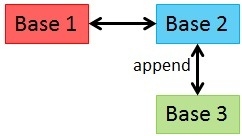
\includegraphics[height=2.7cm]{graf8}
\end{center}
\end{frame}

\begin{frame}{Merge}
\begin{itemize}
\item \textbf{merge} combina observaciones de la base \textit{en memoria} (llamada ``master'') con las observaciones correspondientes de la base en el disco (llamada ``using'') a partir de una o más variables clave
\begin{itemize}
\item \textbf{Caso 1:1}: \textbf{merge 1:1} varlist \textbf{using} \textit{filename}
\item \textbf{Caso 1:m}:  \textbf{merge 1:m} varlist \textbf{using} \textit{filename}
\item \textbf{Caso m:1}:  \textbf{merge m:1} varlist \textbf{using} \textit{filename}
\end{itemize}
\item Ambas bases deben estar ordenadas por varlist (identificador)
\end{itemize}
\end{frame}

\begin{frame}{Merge}
\begin{itemize}
\item Por default se crea una nueva variable \textbf{\_merge} que contiene los códigos numéricos del merge para cada observación
\end{itemize}
\begin{center}
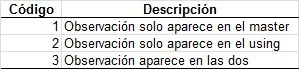
\includegraphics[height=1.7cm]{graf9}
\end{center}
\end{frame}


\begin{frame}{Append}
\begin{itemize}
\item \textbf{append} añade al final de una base en memoria otra base guardada en el disco
\item Si los archivos tienen variables únicas STATA resuleve esto completando con valores \textit{missing} donde es necesario
\end{itemize}
\end{frame}

\section{Variables con subíndice}
\begin{frame}{Variables con subíndice}
\begin{itemize}
\item Se puede hacer referencia a observaciones específicas de una variable a través de subíndices
\item \_n: observación \textit{corriente} y \_N: total de observaciones
\item La mayor parte de los comandos están \textit{vectorizados}. Esto quiere decir que cuando tipeamos
\textbf{\underline{gen}erate} x = y + z STATA interpreta:
{\footnotesize
\[ x[1] = y[1] + z[1]\]
\[ x[2] = y[2] + z[2]\]
\begin{center}
...
\end{center}
\[x[\_N] = y[\_N] + z[\_N]\]}
\item Si en cambio escribimos \textbf{\underline{gen}erate} x = y[1] cada observación de $x$ será igual a la primera observación de $y$  
\item En el marco de [by varlist:] \_n y \_N ser reinterpretan, aplicándose al interior de cada grupo definido por by varlist:
\end{itemize}
\end{frame}

\begin{frame}{Variables con subíndice}{Ejemplo sencillo con by varlist:}
{\footnotesize
\textbf{use} http://www.stata-press.com/data/r11/gxmpl6\\
\textbf{list}\\\gibskip
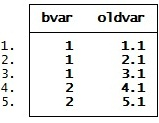
\includegraphics[height=2cm]{graf1.jpg}\\
\textbf{generate} small\_n = \_n\\
\textbf{generate} big\_n = \_N\\
\textbf{generate} newvar = oldvar[1]\\
\textbf{list}}\\\gibskip
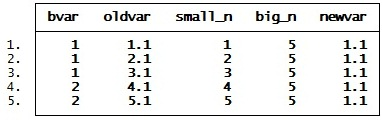
\includegraphics[height=2cm]{graf2.jpg}
\end{frame}

\begin{frame}{Variables con subíndice}{Ejemplo sencillo con by varlist:}
{\footnotesize
\textbf{drop} small\_n big\_n newvar\\
\textbf{bys bvar: generate} small\_n = \_n\\
\textbf{bys bvar: generate} big\_n = \_N\\
\textbf{bys bvar: generate} newvar = oldvar[1]\\
\textbf{list}}\\\gibskip
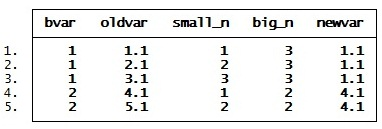
\includegraphics[height=2.2cm]{graf3.jpg}
\end{frame}

\begin{frame}{Etiquetas}
\begin{itemize}
\item Muchas veces es útil usar etiquetas para aclarar el significado de algunas cosas
\item Se pueden asignar etiquetas a:
\begin{itemize}
\item Una base de datos: \textbf{\underline{la}bel \underline{da}ta} \textit{"label"}
\item Una variable: \textbf{\underline{la}bel \underline{var}iable} \textit{varname} \textit{"label"}
\item A los valores que toma una variable  \textbf{\underline{la}bel \underline{val}ues} \textit{varlist} [\textit{"lblname"}] 
\end{itemize}
\item En el último caso primero debemos definir el mapeo
\item Aunque la variable tenga un value label, STATA la sigue considerando una variable numérica 
\end{itemize} 
\medskip
{\footnotesize Ejemplo:}\\
\begin{tabular}{|p{11cm}|}
\hline
{\footnotesize \textbf{label define} repara 1 ``pobre'' 2 ``minima'' 3 ``promedio'' 4 ``buena'' 5 ``excelente''}\\
{\footnotesize \textbf{label values} rep78 repara}\\
\hline
\end{tabular}
\end{frame}


\end{document}


QUEDÓ PENDIENTE: 
Actualización de stata


section{archivos "DO" y "LOG"}

\begin{frame}{Archivos ``DO'' y ``LOG''}
\begin{itemize}
\item Hasta ahora, la interacción con STATA ha sido mediante el tipeo de comandos en la ventana \textbf{``Commands''}
\item A partir de ahora, trabajaremos creando archivos de texto qe contengan toda la secuencia de comandos, esto es, un archivo \textbf{``.DO''}
\item Adicionalmente, los resultados son almacenados en un archivo de texto llamado \textbf{``.LOG''}
\end{itemize}
\end{frame}

\begin{frame}{Archivos do}
\begin{itemize}
\item Son archivos de texto plano que contienen sentencias de STATA que se ejecutan en forma secuencial
\item Es posible editarlos con el editor de STATA, al que se accede mediante el comando \textbf{doedit}, o con editores externos:
\begin{itemize}
\item {\footnotesize \textbf{Editplus}: \url{http://www.editplus.com}}
\item {\footnotesize \textbf{Crimson}: \url{www.crimsoneditor.com}}
\end{itemize}
\item Para crear un archivo do abrimos el editor, escribimos las sentencias que se desean ejecutar y guardamos el archivo con extensión .do en la carpeta de trabajo
\item En los do pueden introducirse comentarios, frases que STATA ignora pero facilitan el entendimiento del código
\item Se consideran comentarios las líneas que empiezan con asterisco (*) o un bloque encerrado entre /* y */
\end{itemize}
\end{frame}

\begin{frame}{Archivos do}
\begin{itemize}
\item Si una sentencia es demasiado larga se puede separar en dos o más líneas agregando /// 
\item El comando \textbf{version} permite especificar cuál es la versión de STATA que estamos utilizando, lo que asegura que el código funcionará si se corre en una versión posterior
\item Se recomienda que los do empiecen con una línea como: \textbf{version} 11.1
\item El comando \textbf{set more off} le dice a STATA que no muestre el mensaje ----more---- y que por lo tanto no haga una pausa en cada pantalla 
\end{itemize}
\end{frame}

\begin{frame}{Ejemplo de un archivo do}
\bigskip
\begin{tabular}{|p{10cm}|}
\hline
\textbf{version} 11.1\\
\textbf{capture log close}\\
\textbf{log using} prueba.log, replace text\\
\textbf{set more off}\\
\textbf{use} \textit{filename}, clear\\
...\\
...\\
\textit{instrucciones}\\
...\\
...\\
\textbf{log close}\\
\textbf{exit}\\
\hline
\end{tabular}\\
\end{frame}

\begin{frame}{Archivos log}
\begin{itemize}
\item Es importante tener una ``memoria'' de la sesión de trabajo. 
\item El archivo \textbf{``.LOG''} guarda los comandos ejecutados y los resultados que se registran en la ventana ``Results''
\item El comando para crear un log es:\\
\bigskip
\begin{tabular}{|p{8cm}|}
\hline
 \textbf{log using} \textit{filename}, text replace\\
\hline
\end{tabular}\\
\bigskip
\item La opción text hace que STATA guarde los registros en un archivo de tipo texto
\item La opción replace implica que los resultados se sobre-escriben. En cambio, la opción append permite grabar corridas sucesivas (poco frecuente)
\end{itemize}
\end{frame}

\begin{frame}{Comandos para crear un log}
\begin{tabular}{|p{6.9cm}|}
\hline
\textbf{capture log close}\\
\textbf{log using} \textit{filename}, text replace\\
\hline
\end{tabular}
\bigskip
\begin{itemize}
\item El comando \textbf{log using} resulta en un error si ya tenemos un log en uso: primero debemos cerrar cualquier otro log con el comando \textbf{log close}
\item El problema es que \textbf{log close} da error si no hay un log en uso
\item Para eso usamos el comando \textbf{capture}
\end{itemize}
\end{frame}



